\documentclass{report}
\usepackage[utf8]{inputenc}
\usepackage{graphicx}
\title{Computer Studies}
\author{Doston Hamrakulov }
\date{February 2018}

\begin{document}
\maketitle

\chapter{First practical work}
\section{Introduction}

Creating a document in LaTeX. LaTeX is a great tool to create documents, it's based on the wysiwym (what you see is what you mean) idea, meaning you only have focus on the contents of your document and the computer will take care of the formatting. With LaTeX is very easy to create professional-looking material

\section{Learning}

sharelatex.com
you open account with programmer2509@gmail.com

so you dont need to install late in your PC, you just can go sharelatex.com and do practical work

\section{Practical work}

Online editor:

1.overleaf.com

2. sharelatex.com



\section{Picture}

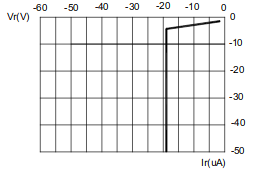
\includegraphics[width=10cm]{First.png}

%============= Second chapter
\chapter{Second practical work}
\section{Introduction}

Creating a document in LaTeX. LaTeX is a great tool to create documents, it's based on the wysiwym (what you see is what you mean) idea, meaning you only have focus on the contents of your document and the computer will take care of the formatting. With LaTeX is very easy to create professional-looking material

\section{Learning}

sharelatex.com
you open account with programmer2509@gmail.com

so you dont need to install late in your PC, you just can go sharelatex.com and do practical work

\section{Practical work}

Online editor:

1.overleaf.com

2. sharelatex.com



\section{Picture}



\end{document}
